%Tender For Computer Science Biometric Access System project (COSBAS)

\documentclass[12pt]{article}

\usepackage{pdflscape}
\usepackage[margin=0.8in]{geometry}
\usepackage{titling}
\usepackage{graphicx}
\usepackage[hidelinks]{hyperref}
\usepackage{color}
\usepackage{framed}
\usepackage{wrapfig}


\graphicspath{ {../images/} }

%If you want to define your own color here is how:
%\definecolor{myOrange}{RGB}{255, 165, 0}

\begin{document}

\begin{titlepage}
	\begin{center}
		
		\begin{figure}[t]
			\centering
			
\includegraphics[width=350px]{UP_Logo.png}
		\end{figure}
		
		%Title
		\textsc{\Huge Project Tender} \\ 

		\textsc{\huge \\Project:\\	}
		\huge Biometric Access System (COSBAS) 
		\textsc{\Large \\Client:}
		\large Department of Computer Science \\

		\textsc{\huge \\ Team:}
		\huge \textsc{\char 60}undecidables\textsc{\char62}
		\begin{flushright} \large
			Elzahn Botha 		\emph{13033922} \newline
			Jason Richard Evans	\emph{13032608} \newline
			Renette Ros			\emph{13007557} \newline
			Szymon Ziolkowski	\emph{12007367} \newline
			Tienie Pritchard 	\emph{12056741} \newline
			Vivian Venter 		\emph{13238435} \newline
\end{flushright}
		\small Department of Computer Science, University of Pretoria \\

	\vfill

	{\large Date: \today}		
		
		
	\end{center}
\end{titlepage}

\newpage
\tableofcontents

\pagebreak

\section{The Team}
% A short description of our team members
% I will add the outline of my description, just copy and paste it over and add your details -> also keep it aplhabetically -> see readMe for order of members

%start of member section
%WITHOUT STUFF THERE IS CHAOS :P 
\subsection{Elzahn Botha}
\begin{wrapfigure}[6]{l}{90px}


\includegraphics[width=80px]{ElzahnBotha.jpg}
\end{wrapfigure}

\textcolor{white}{.}
\subsubsection{Interests}
\begin{itemize}
	\item{Video Games}
	\item{Game development}
	\item{Programming}
	\item{Anime}
\end{itemize}
\subsubsection{Technical Skills} 
\begin{itemize}
	\item{I have already been exposed to Java and been working with it for about a year now}.
	\item{HCI}
	\item{Web development}
\end{itemize}
\subsubsection{Past Experience}
\begin{itemize}
	\item{I have experience in writing programs and systems in Java}.
\end{itemize}
\subsubsection{Non-Technical Strengths} 
\begin{itemize}
	\item{Hard and dedicated worker}
	\item{Always ready to learn new technologies and languages}
	\item{Functions best under pressure}
\end{itemize}
\subsubsection{Why I want to do this project}
This project seemed like it would be a rather interesting project to do as well as the fact that it would be great exposure to a whole new side of IT that I have not yet had the privilege of delving into. I believe that by doing this project I will get valuable exposure that can later help in other projects that I might attempt. This project also seems like it would be a good challenge since I am more comfortable with smaller projects and systems and by doing a larger project such as this it will help me broaden my range of capabilities. Lastly due to the size of the project and the strict time line the pressure will be greatly increased helping me to work at my best without losing interest with the project. 

\pagebreak
\subsection{Jason Richard Evans}
\begin{wrapfigure}[5]{l}{100px}
\vspace{10pt}

\includegraphics[width=80px]{Jason.jpg}
\end{wrapfigure}

\textcolor{white}{.}
\subsubsection{Interests}
\begin{itemize}
	\item{Music Enthusiast}
	\item{Software development}
	\item{Adventure Sports}
\end{itemize}
\subsubsection{Technical Skills}
\begin{itemize}
	\item{C++ and Java}
	\item{Web Development}
\end{itemize}
\subsubsection{Past Experience}
%WHAT SHOULD I WRITE HERE??
Assignments and projects completed for University purposes. A lot of exposure with writing Java applications and servers.
\subsubsection{Non-Technical Strengths}
\begin{itemize}
	\item{Positive outlook on life}
	\item{Hard worker}
	\item{Good team worker}
	\item{An eager learner}
\end{itemize}
\subsubsection{Why I want to do this project}
The field of computer security and the use of biometric systems is extremely interesting to me. I might not have the relevant experience but I know that my persistence and perfectionism will suffice in producing a well planned and valuable product. I am always open to new and exciting challenges and will enjoy this project as such. This project will also give me extremely valuable experience and help me grow as a programmer in software security.

\pagebreak
\subsection{Renette Ros}
\begin{wrapfigure}[8]{l}{90px}

\includegraphics[width=80px]{Renette.jpg}
\end{wrapfigure}
\textcolor{white}{}
\subsubsection{Interests}
\begin{itemize}
	\item Reading
	\item Playing Games
	\item Painting
	\item Puzzles and problem solving
	\item Programming
	\item New interesting technologies
\end{itemize}
\subsubsection{Technical Skills}
\begin{itemize}
	\item Java
	\item C++
	\item Web Development
	\item HCI - User Experience and User interface design
	\item XML, XML Schemas and related technologies.
	\item Good at identifying possible problems and debugging code
\end{itemize}
%\subsubsection{Past Experience}

\subsubsection{Non-Technical Strengths}
\begin{itemize}
	\item Hard Worker
	\item I don't like to do things halfway
	\item I learn new technologies easily
	\item I'm very enthusiastic about things I'm interested in.
\end{itemize}
\subsubsection{Why I want to do this project} 
I want to do this project because I am interested in biometrics and I believe this project has the potential to be very useful in may different settings. I enjoy challenges and I believe this project will help me gain valuable experience in both software engineering and working with multiple different technologies, libraries and APIs. 

\pagebreak
\subsection{Szymon Ziolkowski}
\begin{wrapfigure}[5]{l}{150px}
\vspace{10pt}
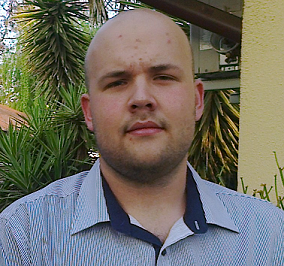
\includegraphics[width=0.24\textwidth]{Szymon.png}
\end{wrapfigure}

\textcolor{white}{.}
\subsubsection{Interests}
	\begin{itemize}
		\item Networks
		\item Security
		\item Computer hardware and electronics
		\item Paintball
		\item Video games
	\end{itemize}
\subsubsection{Technical Skills} 
	\begin{itemize}
		\item C\# and Java
		\item Web development
		\item SQLite, MySQL and SQL Server
	\end{itemize}
\subsubsection{Past Experience}
I have experience in web development and databases that are somewhat relevant to certain aspects of this project.
\subsubsection{Non-Technical Strengths}
	\begin{itemize}
		\item Don't give up easily
		\item Helpful
		\item Determined
	\end{itemize}
\subsubsection{Why I want to do this project} 
I want to do this project because it interests me greatly, it poses many interesting challenges and has a cool factor to it. I have little to no experience in most aspects of this project but this is also the reason why I want to do this project as it will allow me to gain experience and learn new things. 
 

\pagebreak
\subsection{Tienie Pritchard}
\begin{wrapfigure}[7]{l}{150px}
\vspace{10pt}

\includegraphics[width=150px]{Tienie.jpg}
\end{wrapfigure}

\textcolor{white}{.}
\subsubsection{Interests}
\begin{itemize}
	\item{PC Games}
	\item{Music}
		\subitem- Paramore
		\subitem- Flyleaf
		\subitem- Rise Against
	\item{Software Development}
	\item{Series Junkie, including}
		\subitem- The Big Bang Theory
		\subitem- The Vampire Diaries
	\item{Anime}
		\subitem- Naruto
		\subitem- Fairy Tail
\end{itemize}
\subsubsection{Technical Skills}
\begin{itemize}
	\item{Java, including experience in JavaFX and Swing}
	\item{C++}
	\item{General Networking - experience in implementing protocols such as HTTP, POP3 and SMTP}
	\item{Web Development (Advanced)}
		\subitem- HTML4/5
		\subitem- JavaScript
			\subsubitem-- JQuery
			\subsubitem-- NodeJS
		\subitem- CSS3
		\subitem- XML
		\subitem- XSL
			\subsubitem-- XSLT
			\subsubitem-- XSL:FO
		\subitem- PHP
	\item Adobe Suite
		\subitem- Flash CS6/CC
			\subsubitem-- ActionScript 3
		\subitem- Photoshop
		\subitem- Illustrator
		\subitem- Audition
		
\end{itemize}

\subsubsection{Non-Technical Strengths}
\begin{itemize}
	\item{I'm a hard worker and I don't give up easily}
	\item{I'm knowledgeable about general trends in development}
	\item{I'm extremely punctual when it comes to deadlines}
	\item{I'm a fast learner, and I'm willing to learn}
	\item{I'm extremely dedicated to any project I set my mind on}
	\item{I work well in teams}
\end{itemize}
\subsubsection{Past Experience} 
\begin{itemize}
	\item{Two years of experience in writing and implementing Java programs, specifically related to creating data structures and concurrency to achieve various tasks}.
	\item{Two years of experience in writing and implementing C++ programs, including implementation of various design patterns as well as general program design}.
	\item{As part of my Networks module, I have experience in implementing protocols such as HTTP, SMTP and POP3}.
\end{itemize}
\subsubsection{Why I want to do this project}
I believe the opportunity to learn more about how software controls and interacts with external hardware would be amazing. Also, the ability to gain experience with working with biometrics would be invaluable, since I have little to no experience working with it (although I find it very interesting). 


\pagebreak
\subsection{Vivian Laura-Lee Venter}
\begin{wrapfigure}[7]{l}{150px}
\vspace{10pt}

\includegraphics[width=150px]{Vivian.png}
\end{wrapfigure}

\textcolor{white}{.}
\subsubsection{Interests}
\begin{itemize}
	\item{Computer Games}
		\subitem- First Person Shooter
		\subitem- Sport/Soccer
		\subitem- Strategic
	\item{Music And Movies}
	\item{Watching Sports Fanatic: }
		\subitem -Rugby 
		\subitem -Football
		\subitem -Cricket
		\subitem -Athletics
	\item{Software Development/Programming}
	\item{Computer Hardware/Gaming System builds Fanatic }
\end{itemize}
\subsubsection{Technical Skills}
\begin{itemize}
	\item{Java and JavaFX}
	\item{C++}
	\item{Client/Server Applications (Beginner)}
	\item{Web Development (Beginner)}
	\item{Design Patterns}
	\item{Program/System Tester and Debugging}
\end{itemize}

\subsubsection{Non-Technical Strengths}
\begin{itemize}
	\item{Hard-Worker}
	\item{Compationate}
	\item{Competent in knowledgeable/experienced fields}
	\item{Good Listener}
	\item{Diligent}
	\item{Integrity}
	\item{Willing and keen Learner}
	\item{Dedicated to my studies and work}
	\item{Team Player}
	\item{Leader when I need to be}
\end{itemize}
\subsubsection{Past Experience} 
\begin{itemize}
	\item{I have written Java programs and small systems as assignments for my modules at the University of Pretoria}.
	\item{I have written C++ programs and small systems as assignments for my modules at the University of Pretoria}.
	\item{I have written several types of server programs (e.g HTTP) as assignments for my modules at the University of Pretoria}.
\end{itemize}
\subsubsection{Why I want to do this project}
This project is certainly something I have never done before. Being only a novice in biometrics, I am extremely interested in the biometrics aspect of this project. I wanted to do a project where I could learn new, interesting and relevant things. Although this project will be a huge challenge I am willing to dedicate myself and work hard to succeed. 
%end of member section



\section{Project Execution}
% project execution for CMS -> I suggest we discuss this first before adding any sections etc.

\end{document}

